% 足球顶点坐标的计算
% 足球顶点|三棱锥|旋转变换


\pentry{解三棱锥顶角\upref{PrmSol}, 空间旋转矩阵\upref{Rot3D}}

\begin{figure}[ht]
\centering
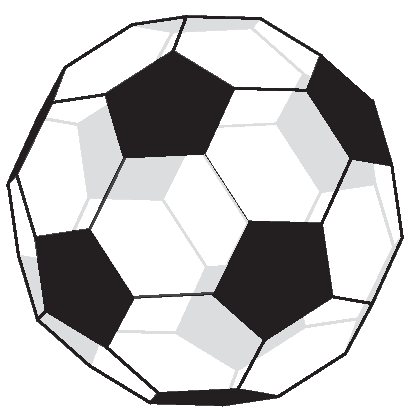
\includegraphics[width=5cm]{./figures/FootBl_1.pdf}
\caption{足球透视图} \label{FootBl_fig1}
\end{figure}

足球的各种常用数据都可以由一个条件推出, 那就是它有 60 个顶点. 考虑到每个顶点都有 3 条同样长度的棱, 棱的个数为
\begin{equation}
(\text{60 个顶点}) \times (\text{3 条棱}) / (\text{每条棱有 2 个顶点}) = 90
\end{equation}
另外每个顶点都由一个正五边形和两个正六边形共用,所以五边形的个数为
\begin{equation}
(\text{60 个顶点}) \times (\text{每个顶点 1 个五边形}) / (\text{每个五边形有 5 个顶点}) = 12
\end{equation}
同理, 六边形的个数为
\begin{equation}
(\text{60 个顶点}) \times (\text{每个顶点 2 个六边形}) / (\text{每个六边形有 6 个顶点}) = 20
\end{equation}

\subsection{坐标计算}
以下所用到的方法不仅适用于足球, 还适用于其他多面体如正十二面体, 正二十面体等. 以足球的一个五边形作为底面, 得到足球的侧视图和俯视图如\autoref{FootBl_fig2}. 为了方便讨论, 我们根据这两个视图把足球的顶点按高度分为 A 到 H 共 8 层.并且逆时针给出相应的数字编号.

\begin{figure}[ht]
\centering
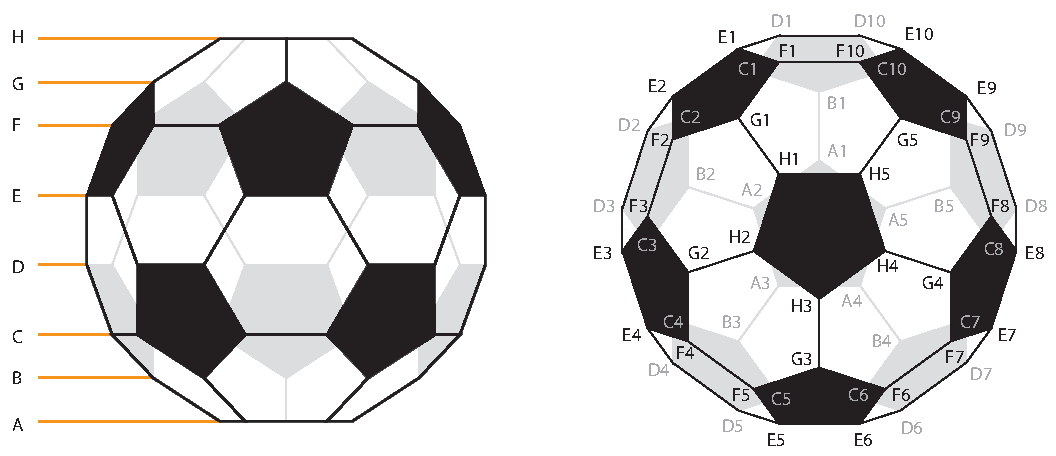
\includegraphics[width=14cm]{./figures/FootBl_2.pdf}
\caption{各层和各顶点的命名, 右图中黑色字体对应五边形的顶点, 灰色字体对应六边形的顶点} \label{FootBl_fig2}
\end{figure}

由于足球由正六边形和正五边形拼成, 足球的每一条棱都相等. 在以下计算中, 不妨设棱长为 1. 通过以下几个步骤, 就可以求解足球的各点的直角坐标.

\subsubsection{求出 $A_1$ 到 $A_5$ 的坐标}
直角坐标系中,令A层的五边形与 $xy$ 平面重合,如下图.为了表示方便,令
\begin{equation}
S = \sin\frac{2\pi}{5} \qquad
C = \cos\frac{2\pi}{5} \qquad
s = \sin\frac{\pi}{5} \qquad
c = \cos\frac{\pi}{5}
\end{equation}
则点 $A_1$ 到 $A_5$ 的坐标分别为
\begin{equation}\label{FootBl_eq5}
\qty(0, \frac{1}{2s}, 0) \quad
\qty(-\frac{S}{2s}, \frac{C}{2s}, 0) \quad
\qty(-\frac12, -\frac{c}{2s}, 0) \quad
\qty(\frac12, -\frac{c}{2s}, 0) \quad
\qty(\frac{S}{2s}, \frac{C}{2s}, 0)
\end{equation}

\subsection{三个重要的角}
由\autoref{PrmSol_eq1}\upref{PrmSol} 可得以下角的大小(以下每个角都是锐角).

两个六边形之间的面面角满足
\begin{equation}
\sin\phi_{66} = \frac{2}{3}
\end{equation}
五边形与六边形之间的面面角满足
\begin{equation}
\sin\phi_{56} = \frac{4s}{\sqrt{15}}
\end{equation}
由\autoref{PrmSol_eq2}\upref{PrmSol}, 五边形与相邻棱的线面角满足 % 未完成: 添加“三棱锥公式”例2并引用
\begin{equation}
\sin\gamma = \frac{2s}{\sqrt5}
\end{equation}

\begin{figure}[ht]
\centering
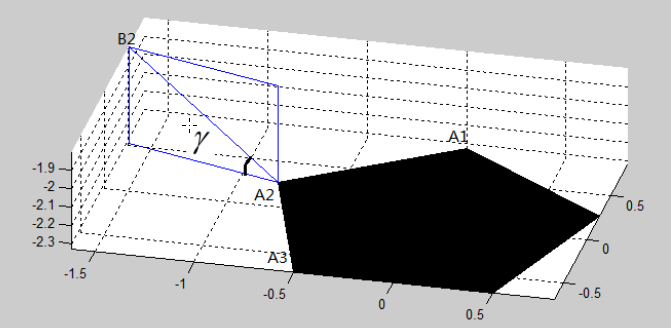
\includegraphics[width=10cm]{./figures/FootBl_4.png}
\caption{求线段 $A_1 B_1$ 与底面的线面角} \label{FootBl_fig4}
% 未完成:图中 B2 改成 B1,用矢量图
\end{figure}

\subsection{求出 $B_1$ 的坐标}

若把从 $A_5$ 指向 $A_1$ 的矢量记为 $\bvec v_1$, $A_2$ 指向 $A_1$ 的矢量记为 $\bvec v_2$, $A_1$ 指向 $B_1$ 的矢量记为 $\bvec u$, 可得
\begin{equation}
\bvec u = \frac{\bvec v_1 + \bvec v_2}{\abs{\bvec v_1 + \bvec v_2}} \cos\gamma
+ \frac{\bvec v_2 \cross \bvec v_1}{\abs{\bvec v_2 \cross \bvec v_1}} \sin\gamma
= \frac{\sqrt{1 - 3S^2/4}}{2s} (\bvec v_1 + \bvec v_2) + \frac{\sqrt{3}}{2} (\bvec v_2 \cross \bvec v_1)
\end{equation}

由\autoref{FootBl_eq5} 得
\begin{equation}
\bvec v_1 = \frac{-S \uvec x + (C-1)\uvec y}{2s} \qquad
\bvec v_2 = \frac{(-S+s)\uvec x + (C+c)\uvec y}{2s}
\end{equation}
代入可得 $\bvec u$ (略), 加上 $A_1$ 的坐标可得 $B_1$ 的坐标. 接下来我们并不需要用同样的方法求出 B 层的其他坐标, 因为我们可以通过一个简单的矢量公式依次求出剩下所有顶点的坐标.

\subsection{求剩下的坐标}
已知空间中正 $N$ 边形任意连续 3 点的坐标, 求第 4 点的坐标, 可以用以下矢量公式来计算
\begin{equation}\label{FootBl_eq9}
\bvec r_4 = \bvec r_1 - \bvec r_2 + \bvec r_3 + 2\sin(\frac{N-4}{2N}\pi) \cdot (\bvec r_3  - \bvec r_2)
\end{equation}
其中 $\bvec r_i$ 是第 $i$ 点的位置矢量\upref{Disp}.

根据已知的 $A_2, A_1, B_1$ 三个点,该式可以算出 $C_1$ 的坐标, 再把 $A_1, B_1, C_1$ 的坐标代入得到 $C_2$, 再由 $B_1, C_1, C_2$ 得到 $B_2$, 以此类推. 当 $C$ 层完成后,又可以同理算出其他层的所有顶点.下面我们来推导这个公式.

\begin{figure}[ht]
\centering
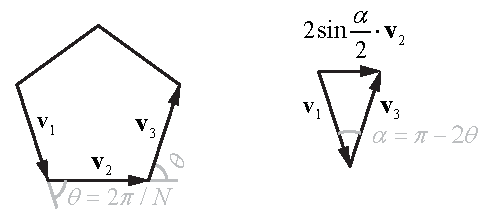
\includegraphics[width=8.3cm]{./figures/FootBl_3.pdf}
\caption{由正 $N$ 边形的 3 个顶点坐标求第 4 个顶点坐标. 图中以五边形为例,但图中的公式适用于任意的 $N > 2$} \label{FootBl_fig3}
\end{figure}

令 $\bvec v_i = \bvec r_{i+1} - \bvec r_i$, 从\autoref{FootBl_fig3} 中不难发现
\begin{equation}
\bvec v_1 + \bvec v_3 = 2\sin(\frac{N-4}{2N}\pi) \cdot \bvec v_2
\end{equation}
将 $\bvec r_i$ 代入即可得到\autoref{FootBl_eq9}.

% 未完成:推导
\subsection{足球的高度和中点坐标}
我们从底部的五边形出发,沿着任意一条外接棱的方向前进,依次会经过棱,五边形,六边形,六边形,顶部的五边形.如果从反方向出发,顺序恰好相反.这两条路线恰好可以绕足球一整圈.
%图未完成,把图二左绕 z 轴旋转一下,使轮廓变为路线

按照第一种路线到达顶部,转过的角度依次是 $\gamma, \gamma, \phi_{56}, \phi_{66}, \phi_{56}$. 可以验证,它们相加等于 $\pi$.%未完成:可以解析验证吗?

考虑到经过的五边形(边长为 1)的中轴线长度是 $(1+c)/(2s)$, 经过的六边形的中轴线长度是 $\sqrt{3}$,经过的棱长为 1,底部五边形到顶部五边形的高度为\footnote{事实上这个式子很难化简,结果来自 \href{https://en.wikipedia.org/wiki/Truncated_icosahedron}{Wikipedia} 查找并通过数值验证.}
\begin{equation}\ali{
h &= \sin\gamma + \frac{1+c}{2s} \sin(2\gamma) + \sqrt{3} \sin(2\gamma + \phi_{56}) + \sqrt{3} \sin(2\gamma + \phi_{56} + \phi_{66})\\
&= \sqrt{\frac{41}{10}\sqrt 5 + \frac{25}{2}}
}\end{equation}
球心到底面和顶面的距离为 $h/2$.

由勾股定理可以得到中心点到任意顶点的距离为
\begin{equation}
R = \sqrt{\qty(\frac{h}{2})^2 + \qty(\frac{1}{2s})^2} = \frac14 \sqrt{18\sqrt{5} + 58}
\end{equation}

%可以列出每个顶点坐标的解析式,再说明如何用旋转矩阵进行旋转

% 未完成:使用球坐标会不会方便一点?

